\documentclass{beamer}\usepackage{graphicx, color}
%% maxwidth is the original width if it is less than linewidth
%% otherwise use linewidth (to make sure the graphics do not exceed the margin)
\makeatletter
\def\maxwidth{ %
  \ifdim\Gin@nat@width>\linewidth
    \linewidth
  \else
    \Gin@nat@width
  \fi
}
\makeatother

\IfFileExists{upquote.sty}{\usepackage{upquote}}{}
\definecolor{fgcolor}{rgb}{0.2, 0.2, 0.2}
\newcommand{\hlnumber}[1]{\textcolor[rgb]{0,0,0}{#1}}%
\newcommand{\hlfunctioncall}[1]{\textcolor[rgb]{0.501960784313725,0,0.329411764705882}{\textbf{#1}}}%
\newcommand{\hlstring}[1]{\textcolor[rgb]{0.6,0.6,1}{#1}}%
\newcommand{\hlkeyword}[1]{\textcolor[rgb]{0,0,0}{\textbf{#1}}}%
\newcommand{\hlargument}[1]{\textcolor[rgb]{0.690196078431373,0.250980392156863,0.0196078431372549}{#1}}%
\newcommand{\hlcomment}[1]{\textcolor[rgb]{0.180392156862745,0.6,0.341176470588235}{#1}}%
\newcommand{\hlroxygencomment}[1]{\textcolor[rgb]{0.43921568627451,0.47843137254902,0.701960784313725}{#1}}%
\newcommand{\hlformalargs}[1]{\textcolor[rgb]{0.690196078431373,0.250980392156863,0.0196078431372549}{#1}}%
\newcommand{\hleqformalargs}[1]{\textcolor[rgb]{0.690196078431373,0.250980392156863,0.0196078431372549}{#1}}%
\newcommand{\hlassignement}[1]{\textcolor[rgb]{0,0,0}{\textbf{#1}}}%
\newcommand{\hlpackage}[1]{\textcolor[rgb]{0.588235294117647,0.709803921568627,0.145098039215686}{#1}}%
\newcommand{\hlslot}[1]{\textit{#1}}%
\newcommand{\hlsymbol}[1]{\textcolor[rgb]{0,0,0}{#1}}%
\newcommand{\hlprompt}[1]{\textcolor[rgb]{0.2,0.2,0.2}{#1}}%

\usepackage{framed}
\makeatletter
\newenvironment{kframe}{%
 \def\at@end@of@kframe{}%
 \ifinner\ifhmode%
  \def\at@end@of@kframe{\end{minipage}}%
  \begin{minipage}{\columnwidth}%
 \fi\fi%
 \def\FrameCommand##1{\hskip\@totalleftmargin \hskip-\fboxsep
 \colorbox{shadecolor}{##1}\hskip-\fboxsep
     % There is no \\@totalrightmargin, so:
     \hskip-\linewidth \hskip-\@totalleftmargin \hskip\columnwidth}%
 \MakeFramed {\advance\hsize-\width
   \@totalleftmargin\z@ \linewidth\hsize
   \@setminipage}}%
 {\par\unskip\endMakeFramed%
 \at@end@of@kframe}
\makeatother

\definecolor{shadecolor}{rgb}{.97, .97, .97}
\definecolor{messagecolor}{rgb}{0, 0, 0}
\definecolor{warningcolor}{rgb}{1, 0, 1}
\definecolor{errorcolor}{rgb}{1, 0, 0}
\newenvironment{knitrout}{}{} % an empty environment to be redefined in TeX

\usepackage{alltt}

\usepackage{amsmath}
\usepackage{graphicx}
\usepackage{microtype}

\DisableLigatures{encoding = *, family = *}
\frenchspacing

\mode<beamer>{
\usetheme{default}
\usecolortheme{orchid}
\setbeamertemplate{navigation symbols}{}
}
\mode<handout>{
\usepackage{pgfpages}
\pgfpagesuselayout{4 on 1}[a4paper, border shrink=10mm, landscape]
\usetheme{default}
}


\title{Reading and Interpretation of the Ten Statistical Commandments of Chairman Alroy}
\subtitle{}
\author{Peter D Smits \inst{1} \inst{2}}
\institute{
\inst{1}
School of Biological Sciences\\
Monash University
\and
\inst{2}
Committee on Evolutionary Biology\\
University of Chicago
}
\scriptsize{\date{\today}}


\begin{document}

\mode*
\begin{frame}
\titlepage
\end{frame}



\begin{frame}
\frametitle{John Alroy}
\begin{columns}
\begin{column}{0.5\textwidth}
\begin{itemize}
\item quantitative paleobiologist currently at Macquarie
\begin{itemize}
\item diversity curves
\item PaleoDB
\end{itemize}
\item teaches quantitative methods in (paleo)biology workshop
\end{itemize}
\end{column}
\begin{column}{0.5\textwidth}
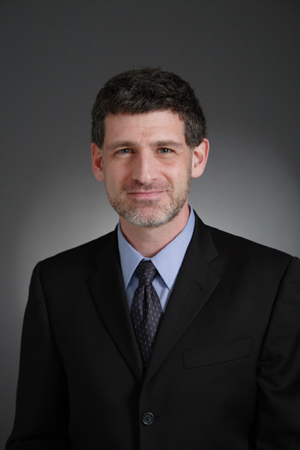
\includegraphics[width = \textwidth, keepaspectratio = true]{dr_john_alroy}
% image is from macquarie website
% www.mq.edu.au
\end{column}
\end{columns}
\end{frame}



\begin{frame}
\frametitle{Background}
John Alroy is (in)famous for getting extremely angry about the use of statistical methods in paleontology (and biology in general.)
\\~\\
Up until about 2-3 years ago he had a list of 10 statistical commandments on his NCEAS website. 
Currently he only lists an abbreviated version. % put a screengrab of it
\\~\\
They are one of the few things I have displayed at my desk.
\\~\\
While the content is serious, the presentation is parody.
\end{frame}



\begin{frame}
\frametitle{}
\begin{columns}
\begin{column}{0.5\textwidth}
The other picture at my desk\dots
\end{column}
\begin{column}{0.5\textwidth}
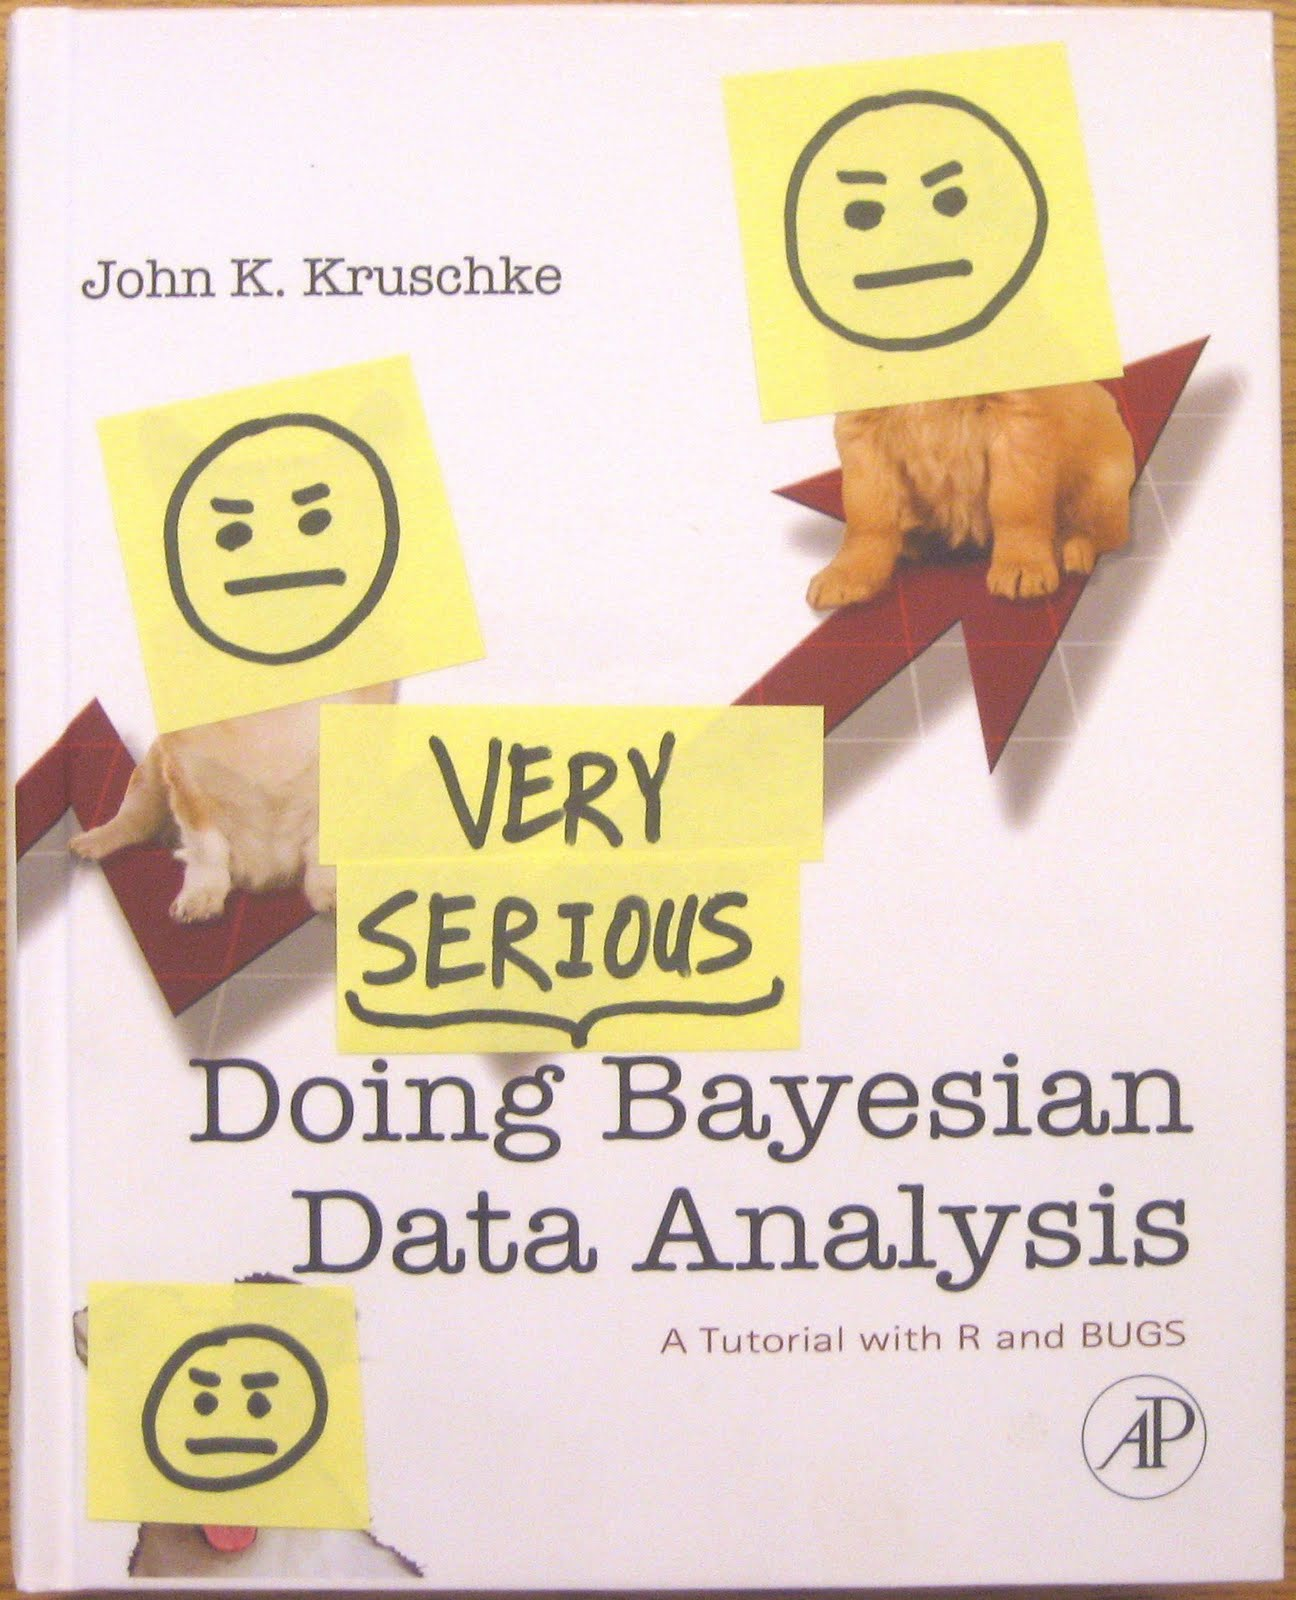
\includegraphics[width = \textwidth]{bayesian}
% image is from john kruschke's blog
% doingbayesiandataanalysis.blogspot.com
\end{column}
\end{columns}
\end{frame}



\begin{frame}
\frametitle{}
\begin{columns}
\begin{column}{0.5\textwidth}
\huge{And Our Beloved Chairman Alroy said \ldots}
\end{column}
\begin{column}{0.5\textwidth}
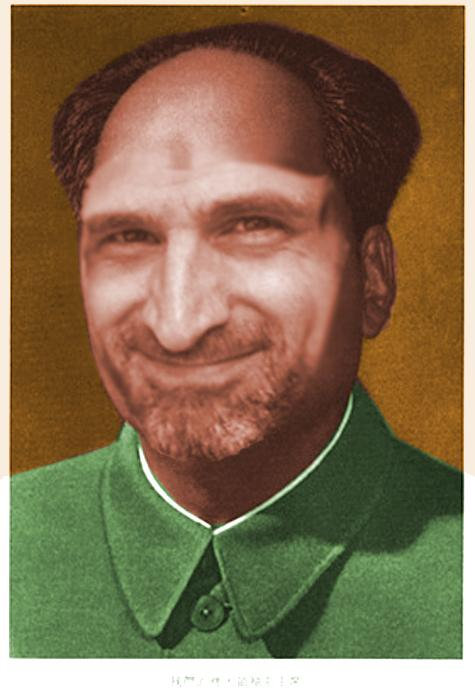
\includegraphics[width = \textwidth, keepaspectration = true]{alroy_mao}
% image is from Dave Polly's slides at the PBDB workshop
\end{column}
\end{columns}
\end{frame}


\begin{frame}
\frametitle{Commandment 1}
\textbf{Thou shalt log thy data! }
We live in a multiplicative world, which means our data live in a log world. 
Always log any data with a lower zero bound, unless there's also an upper bound, 
in which case that shalt perform a logit transformation. 
\emph{Log until proven linear, and be holy.}
\end{frame}


\begin{frame}
\frametitle{Monotonic transform}

% pantheria data
% see pantheria database for information
\begin{knitrout}
\definecolor{shadecolor}{rgb}{0.969, 0.969, 0.969}\color{fgcolor}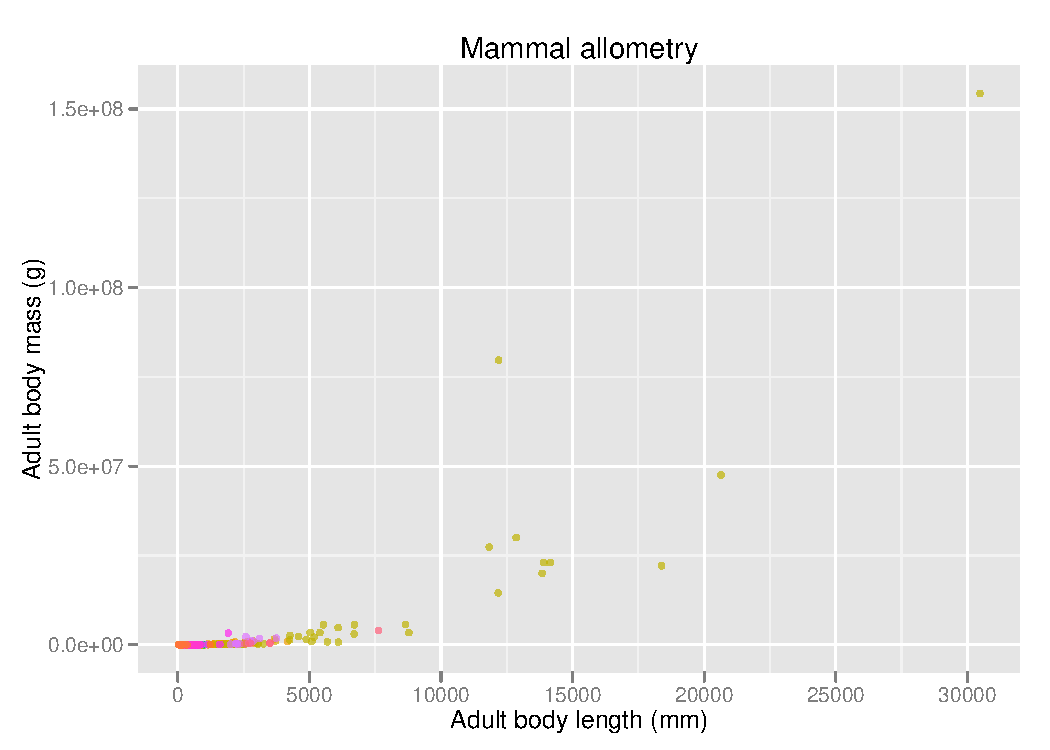
\includegraphics[width=\maxwidth]{figure/body-sze} 
\end{knitrout}

\end{frame}


\begin{frame}
\frametitle{Monotonic transform}

\begin{knitrout}
\definecolor{shadecolor}{rgb}{0.969, 0.969, 0.969}\color{fgcolor}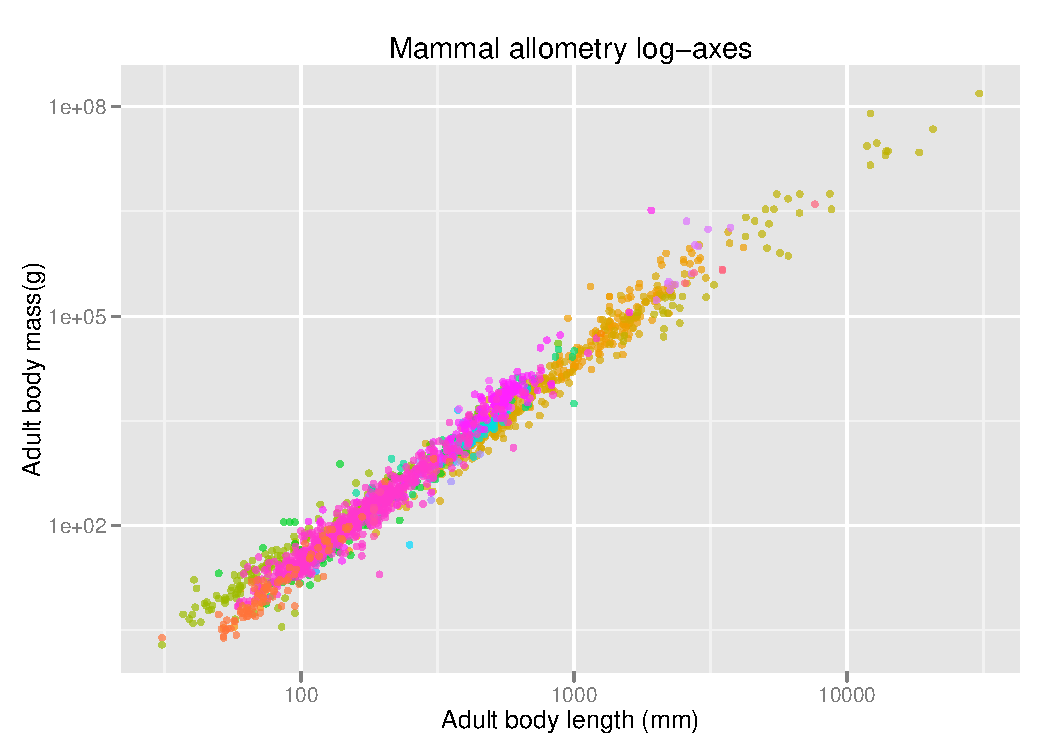
\includegraphics[width=\maxwidth]{figure/body-sze-log} 
\end{knitrout}

\end{frame}


\begin{frame}
\frametitle{Information and log}
Imagine we have a device that can give us one of three items at a time: 

A B C
\\~\\
Everytime we get something from the device, we receive information and our uncertainty decreases.
\\~\\
We can say this device as ``uncertainty 3''
\end{frame}


\begin{frame}
\frametitle{Information and log}
Now imagine a second device that gives one of two items at a time (uncertainty 2): 

Y Z
\\~\\
If we put both devices together, we have six possibilities:

AY AZ BY BZ CY CZ
\\~\\
Even though we have two ``devices.''
\\~\\
The easy way to just do this is take the log of the uncertainty of both ``devices.'' Can contiue from here to explain Shannon's entropy (I won't).
\\~\\
\(\log 3 + \log 2 = \log 6\)
\end{frame}


\begin{frame}
\frametitle{Commandment 2}
\textbf{Thou shalt run non-parametric tests! }
If the parametric and non-parametric tests come out the same, thou hast lost nothing. 
If they don't, the data are non-normal, the parametric test is wrong, and thou shalt use the non-parametric result. 
\underline{Spearman}, \underline{Mann-Whitney}, and \underline{Kolmogorov-Smirnov} are the \underline{Holy Trinity} (or Quintinity, or whatever). 
Worship them!
\end{frame}


\begin{frame}
\frametitle{Non-parametric tests}
Parametric tests have a number of assumptions (normality).
Even the basic Pearson's product-momment of correlation (\(r\)) assumes normality.
\\~\\
Frequently, these assumptions are either un-tested (homogeneity of variance)
or violated (independence).
\\~\\
Very rarely in real systems can most tests be applied. 
Life doesn't always fit in that box.
\\~\\
Non-parametric tests avoid (most) of the problems revolving around distributions.
\end{frame}


\begin{frame}
\frametitle{Non-parametric tests}
Non-parametric statistics, specifically the tests, come in two flavours

\begin{itemize}
\item distribution free
\item non-parametric (I love tautologies)
\end{itemize}

Some examples...
\end{frame}


\begin{frame}
\frametitle{Non-parametric tests}

Spearman rank order coeffecient rho (\(\rho\)) and Kendall's tau (\(\tau\))
\begin{itemize}
\item similar to \(r\) but is based on ranks and, thus, distribution free
\item choice of \(\rho\) or \(\tau\) depends mostly on sample size
\end{itemize}
Wilcox signed-rank test and Mann-Whitney U
\begin{itemize}
\item similar to \(t\)-test but is based on ranks and is for difference of medians (not means). 
\item Wilcox is an alternative to paired \(t\)-test
\item Mann-Whitney is an alternative to two-sample \(t\)-test.
\end{itemize}
Kolmogorov-Smirnov test
\begin{itemize}
\item Did a sample come from a specific probability distribution (one-sample) or did two samples come from the same probability distribution?
\item the two-sample is really unique and incredibly useful
\end{itemize}
\end{frame}


\begin{frame}
\frametitle{Resampling methods}
Missing from the commandment are resampling methods.
\\~\\
Resampling methods (can) have even fewer assumptions than non-parametric methods!
\\~\\
In general, you just assume your sample is representative of the population which we do this almost implicitly.
\\~\\
Resampling methods are various classes of Monte Carlo methods (randomized) and are generally considered computer intensive.
\end{frame}


\begin{frame}
\frametitle{Resampling methods}
% need to edit this image
% left bottom right top
\centering 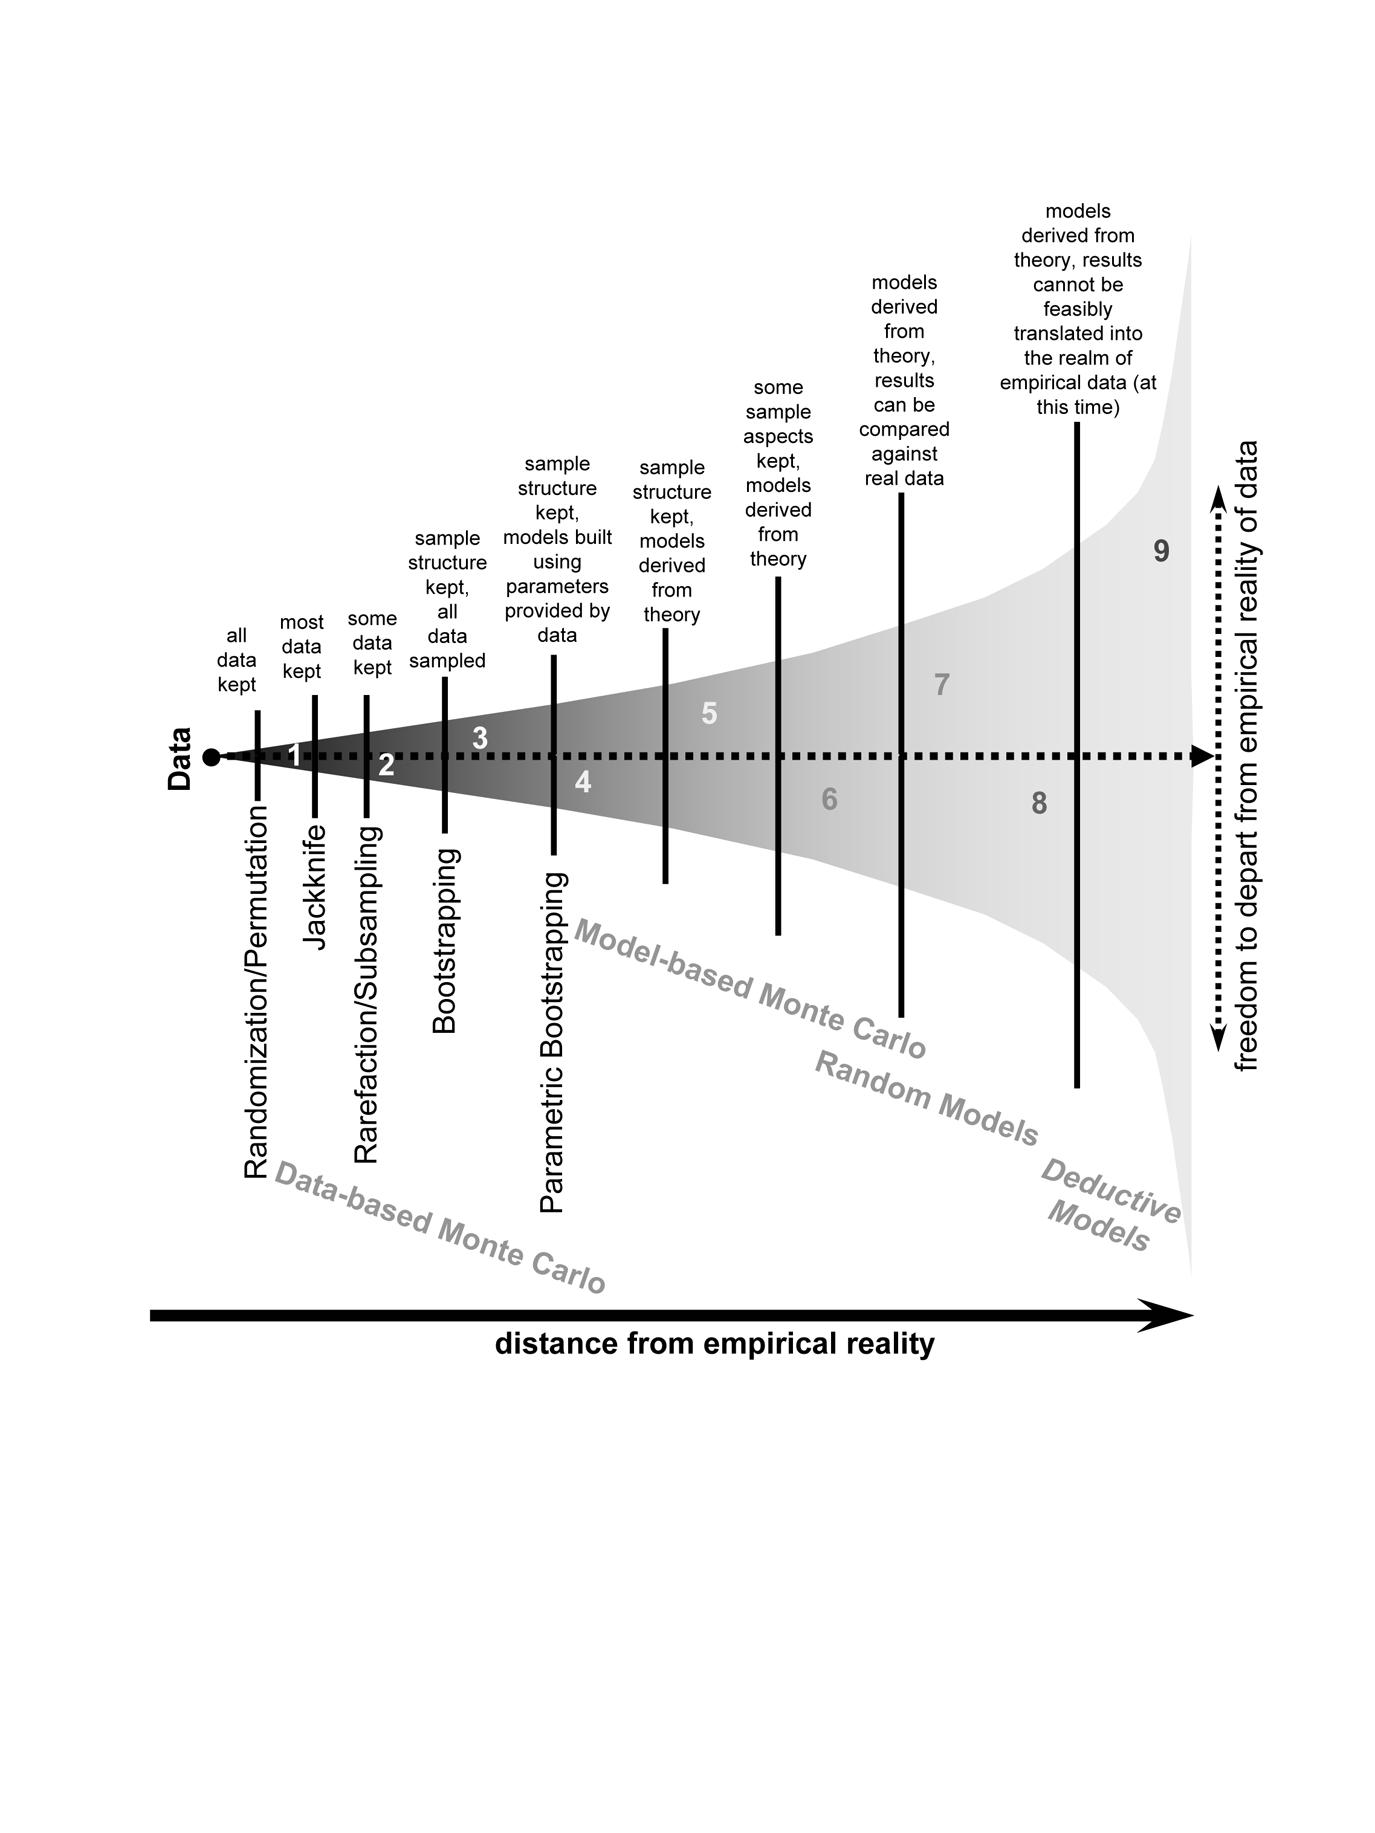
\includegraphics[trim = 0pt 250pt 0pt 85pt, height = 200pt, keepaspectratio = true]{reality}

% need to find a way to put this in bottom right corner
\footnotesize{from Kowalewski and Novack-Gottshall 2010}
\end{frame}


\begin{frame}
\frametitle{Commandment 3}
\textbf{Thou shalt disdain p-values! }
p = 0.05 is a heathen idol, and ANOVAs are for those who have not yet seen the light, still dwelling in the darkness of obsessive frequentist hypothesis testing. 
Remember, \emph{if thou hast enough data anything will turn significant, no matter how small the difference.} 
And the ``significance level'' is whatever thou choosest it to be, not what someone tells thee it should be. 
So, describe data, don't just test data. 
Don't merely ask \emph{whether} there's a significant difference, ask \emph{what} is the difference, \emph{why} is there a difference, and \emph{have I confidence} in that difference?
\end{frame}


\begin{frame}
\frametitle{Definition}
A \(p\)-value is the probability of a result given that the null is true.

Many misconceptions and problems
\begin{itemize}
\item statement of \(P(x | H0)\), not \(P(H1 | x)\) or \(P(H0 | x)\)
\item trivial null hypotheses abound
\item false significant/not significant binary
\item may reflect large sample size rather than anything meaningful
\item etc\ldots
\end{itemize}
\end{frame}


\begin{frame}
\frametitle{p-values}
\(p\)-values are the target of near constant attack.
\\~\\
Part of this has to do with confusing Fisher's original definition and Neyman-Pearson Type I and Type II error rates (I won't discuss this).
\\~\\
John Myles White (sociology grad-student and consumate Bayesian) has been producing a nice series about the problems of the NHST paradigm that touches on the above points: worker effort and effect size.
\end{frame}


\begin{frame}
\frametitle{worker effort}
If effect size \(>\) 0, there exists a large enough sample to be ``significant.''

\begin{knitrout}
\definecolor{shadecolor}{rgb}{0.969, 0.969, 0.969}\color{fgcolor}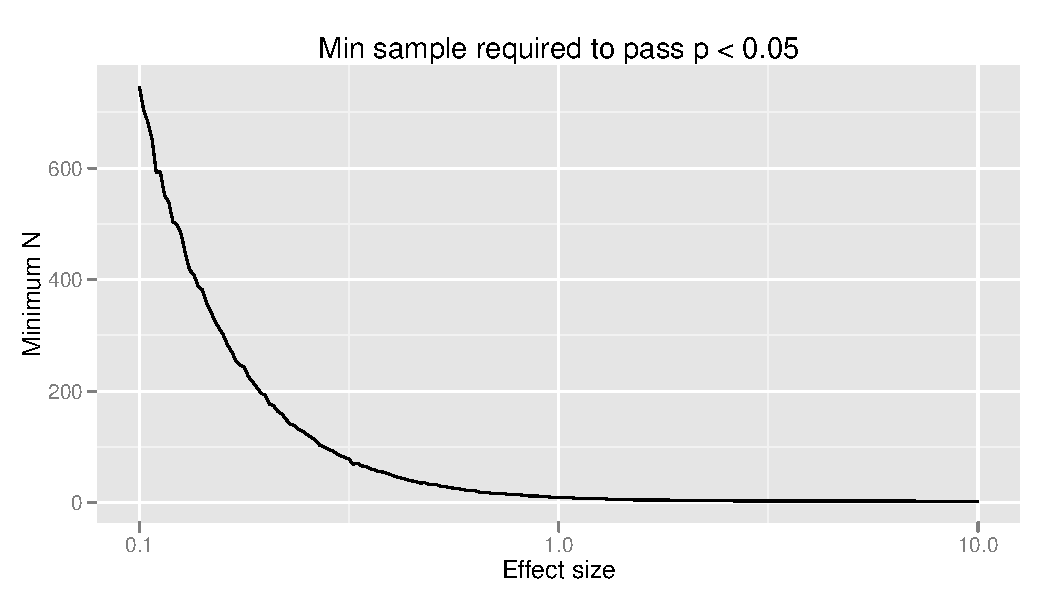
\includegraphics[width=\maxwidth]{figure/jwm-revpower} 
\end{knitrout}

% data is from John Myles White's github
% https://github.com/johnmyleswhite/NHSTExamples

\footnotesize{from JWM's blog, code on github}
\end{frame}


\begin{frame}
\frametitle{Reduction of dimensionality}

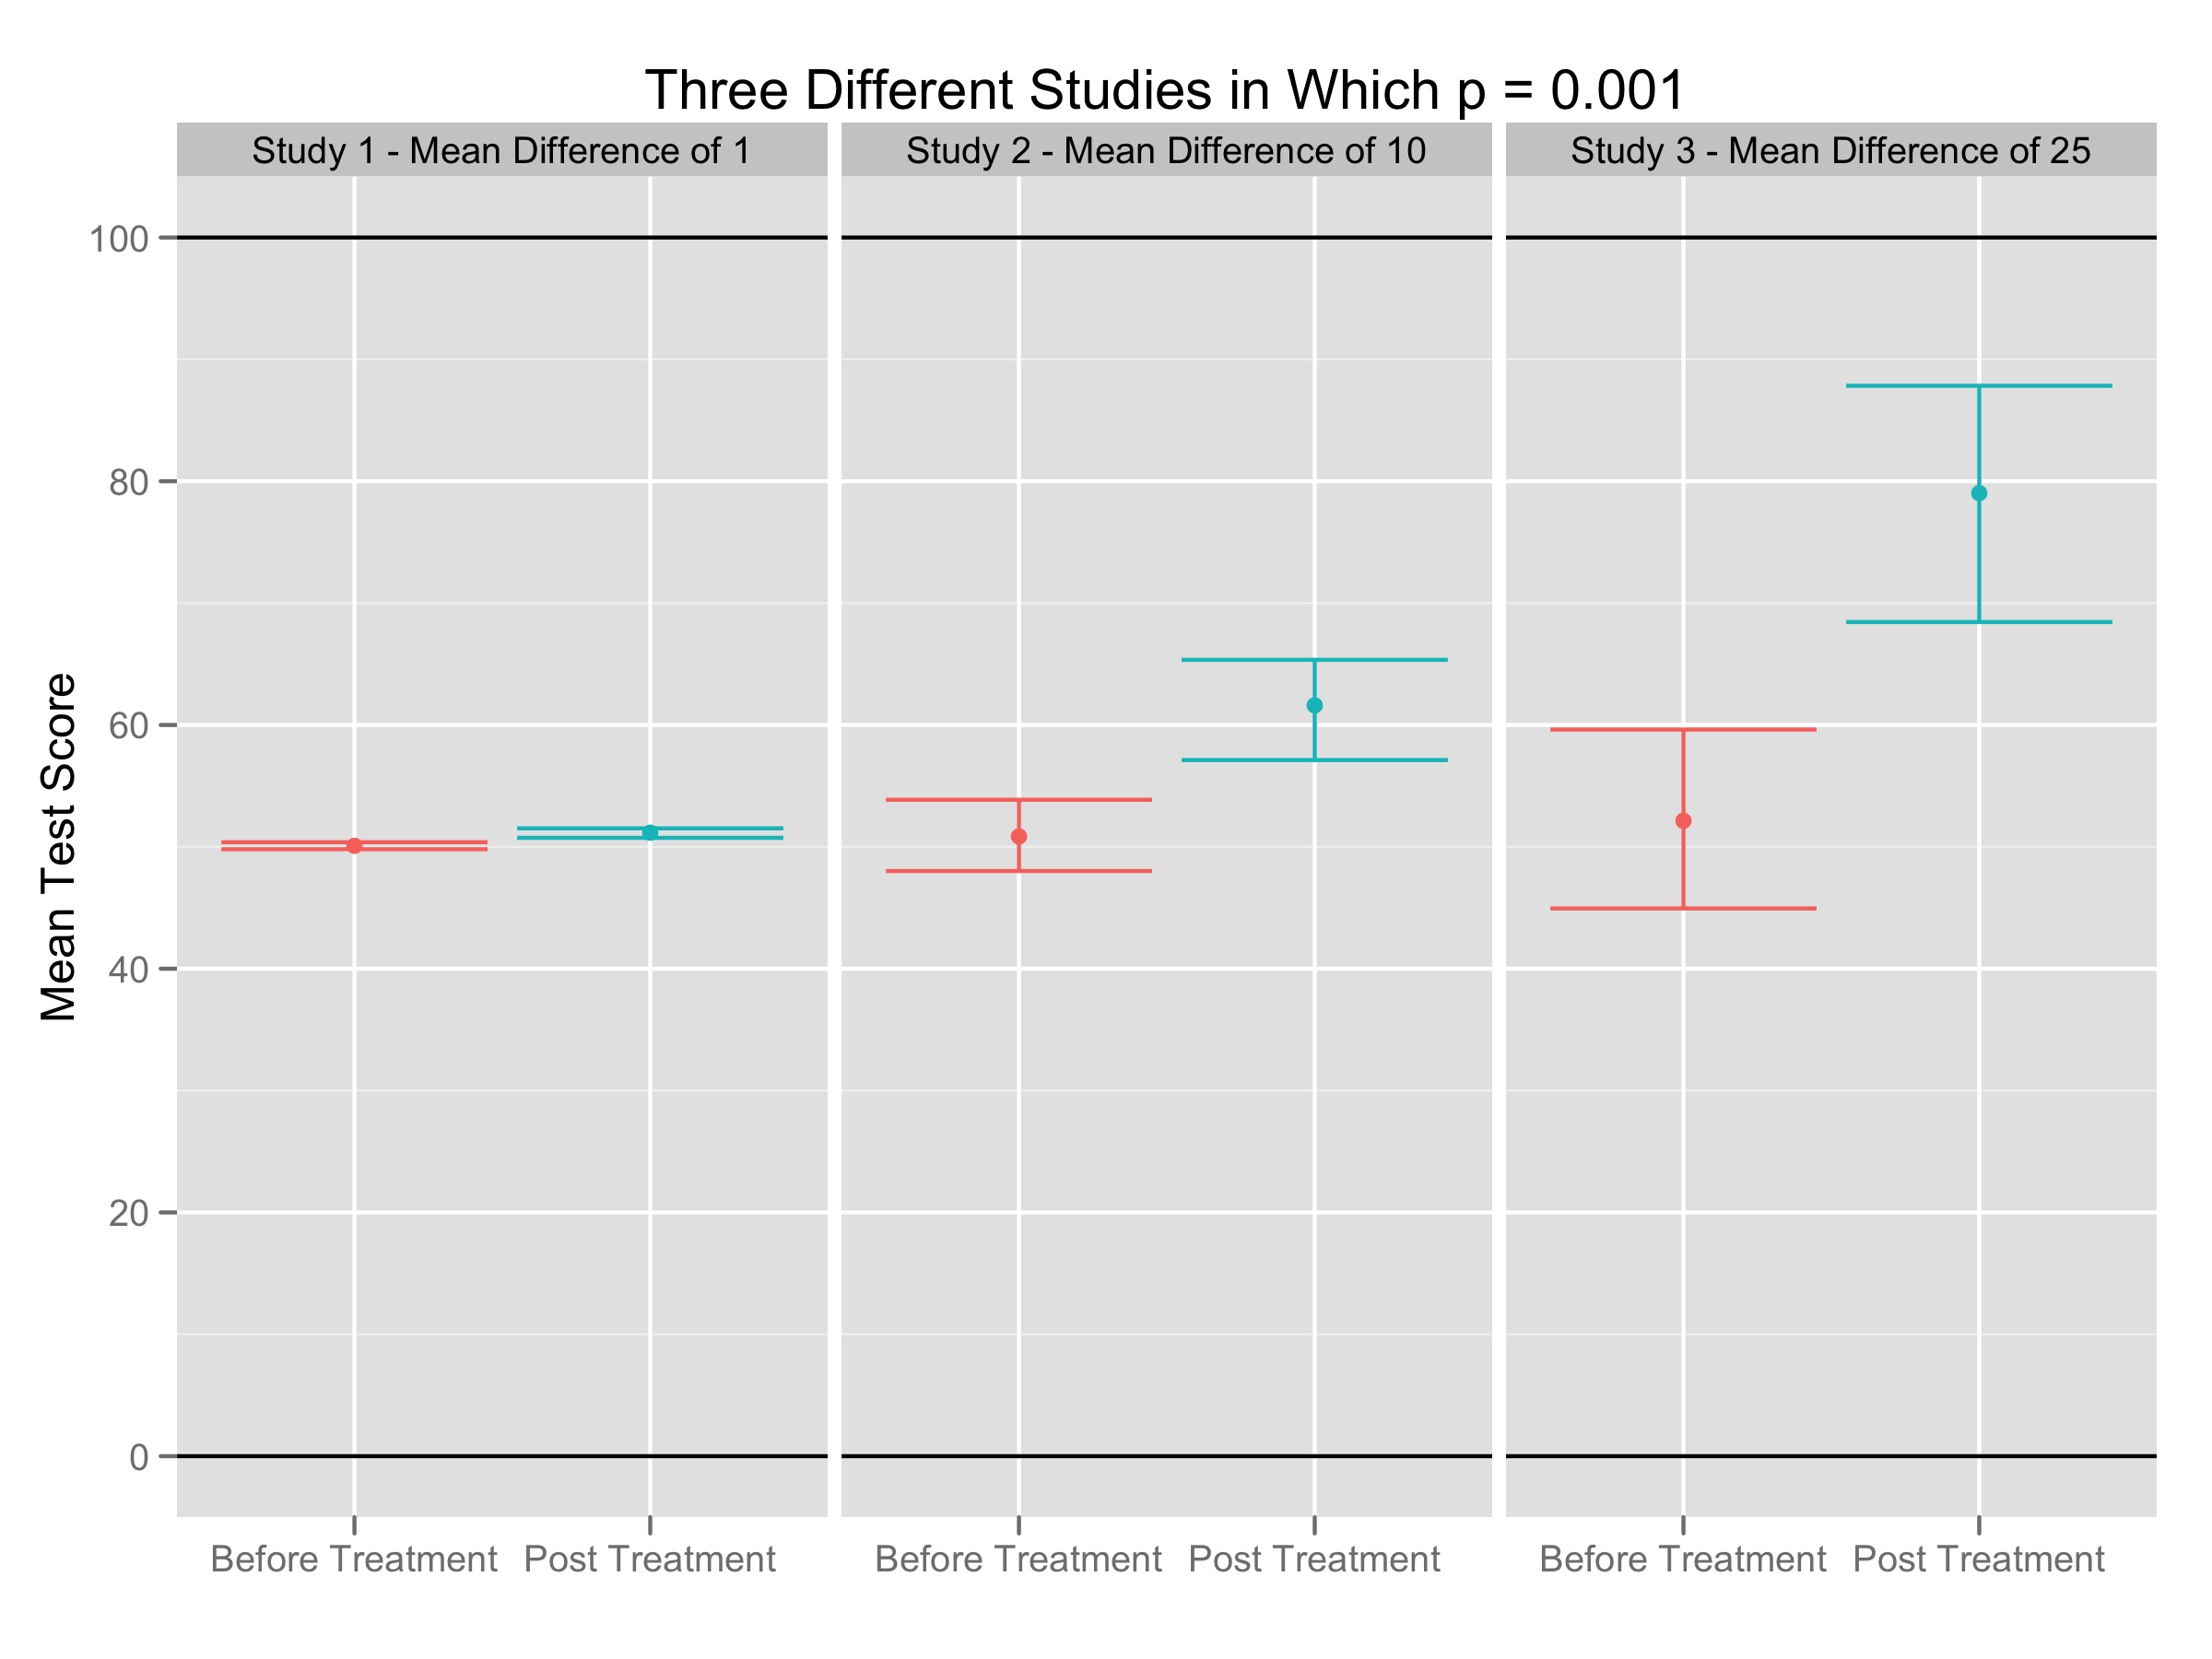
\includegraphics[width = 0.9\textwidth, keepaspectratio = true]{three_studies1}
% from JWM's blog
% http://www.johnmyleswhite.com/

\footnotesize{from JWM's blog}
\end{frame}


\begin{frame}
\frametitle{Comrade Polly}

\begin{flushright}
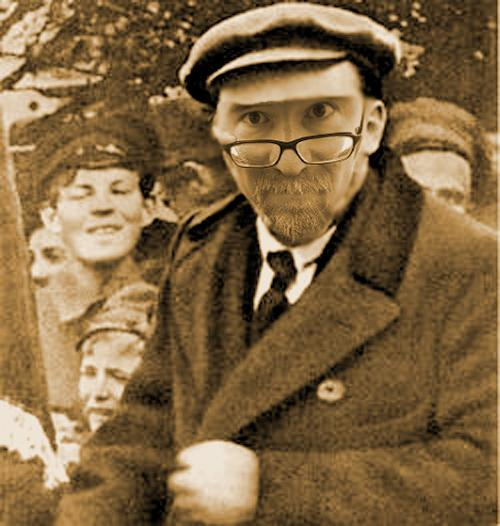
\includegraphics[height = 100pt, keepaspectratio = true]{polly}
% image is from Dave Polly's slides for the PBDB workshop
\end{flushright}

\textbf{Believe what Chairman Alroy says about \(p\)-values!}
But you can still use ANOVA to test for differences in means, though believe what our Beloved Chairman says about asking what is the difference, why is it, and do I believe it!
\end{frame}


\begin{frame}
\frametitle{Take home message}
\Large{``Significance'' is a product of interpretation, not of rigid rules.}
\\~\\
\Large{Statistical inference is concerned with the ``art of approximation''} \small{(Akaike)}.
\end{frame}


\begin{frame}
\frametitle{Commandment 4}
\textbf{Thou shalt worship the almighty power! }
Despite the preceding commandment, accepting the null hypothesis is a vile, ungodly thing. 
Always make sure thou hast the statistical power and \emph{a small enough difference relative to what thou carest about} to argue that a difference doesn't matter (not just that it isn't ``significant''). 
When in doubt, find a power calculator on the web and do a proper power analysis.
\end{frame}


\begin{frame}
\frametitle{Commandment 5}
\textbf{Thou shalt abhor tiny little time series! }
All too often people are seduced by ``trends'' of two or three data points, damning themselves to eternal hellfire. 
The two-tailed probability of a flawless ``trend'' with six points is 0.0625 (!). 
``Before'' and ``after'' comparisons are no better than a single coin flip, unless the points in each category have significantly different averages. 
Coincidences are often coincidences: if (say) the biggest extinction happened in the same interval as the biggest climate change, and there are ten intervals, well, \(p\) = 0.10. 
So, demand that a time series analysis include a healthy number of data points, at least a dozen or a score or a cubit.
\end{frame}


\begin{frame}
\frametitle{Commandment 6}
\textbf{Thou shalt difference thy data! }
Time series data are almost always autocorrelated (and thou shalt test for that). 
Still, people insist on interpreting ``trends'' shared by pairs of time series as meaningful cross-correlations, even though autocorrelation makes finding these demonic things \emph{the null hypothesis!} 
Even random walks produce such patterns! FEAR YE SINNERS! 
The easiest and most powerful way to remove the autocorrelation is to take first differences. 
So, the next time thou wantest to correlate population growth with the rate of sea-floor spreading - and people will - \emph{difference thy \%\!\@\#\$\% data}.
\end{frame}


\begin{frame}
\frametitle{Commandment 7}
\textbf{Thou shalt not play with PCA!} 
Principal components analysis assumes linear responses of observed variables to underlying variables, but most ecological data show modal responses. 
Vain mortal, what power grants thee the right to assume linearity? 
Correspondence analysis can handle both kinds of responses and works wonderfully on modal data (we won't mention that nasty little arch effect...).
\end{frame}


% do i need to explain this data a little before launching in?
\begin{frame}
\frametitle{PCA}

% data is from the PBDB
\begin{knitrout}
\definecolor{shadecolor}{rgb}{0.969, 0.969, 0.969}\color{fgcolor}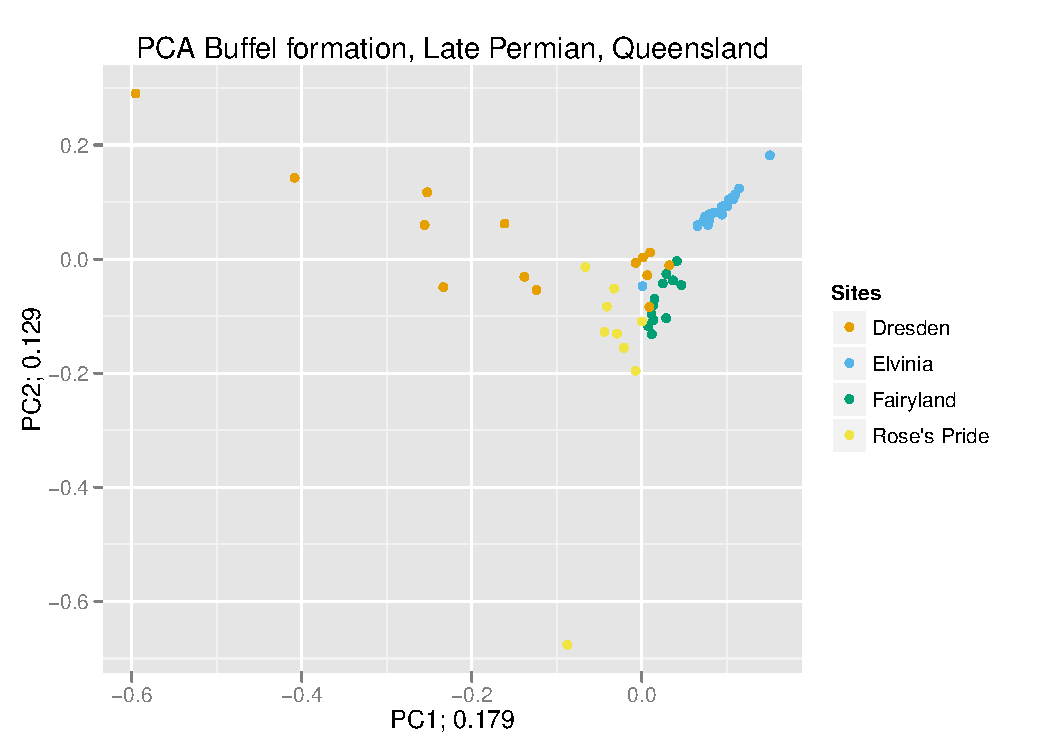
\includegraphics[width=\maxwidth]{figure/buffel-pca} 
\end{knitrout}



\end{frame}


\begin{frame}
\frametitle{CA}

\begin{knitrout}
\definecolor{shadecolor}{rgb}{0.969, 0.969, 0.969}\color{fgcolor}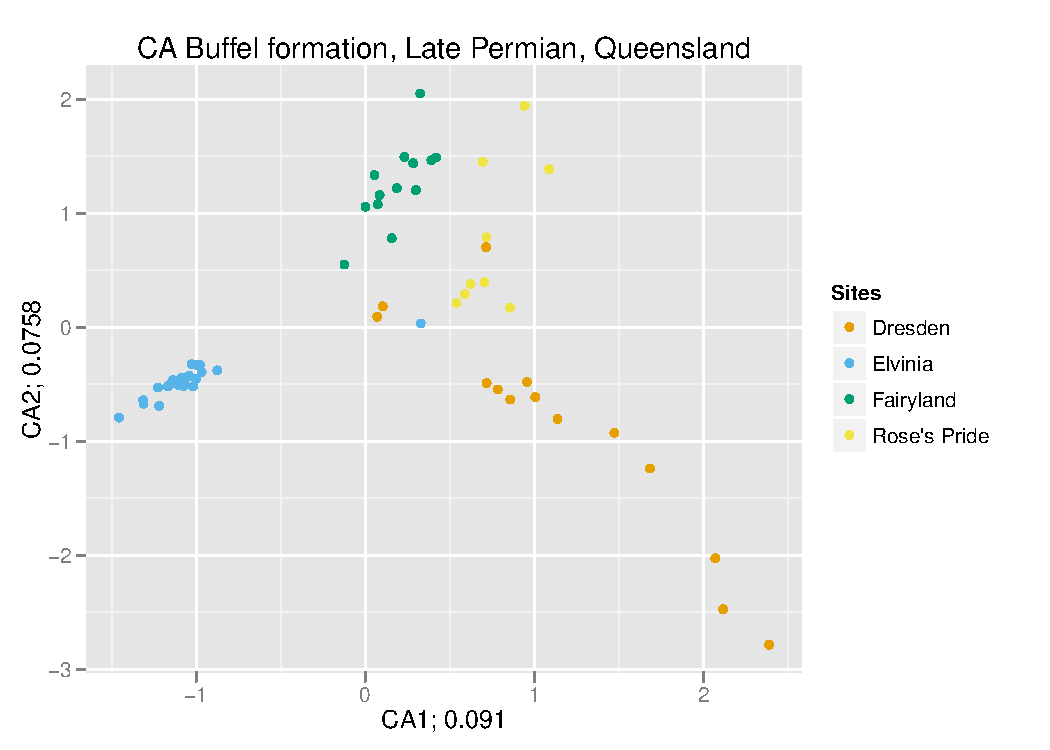
\includegraphics[width=\maxwidth]{figure/buffel-ca} 
\end{knitrout}


\end{frame}



\begin{frame}
\frametitle{PCoA}

\begin{knitrout}
\definecolor{shadecolor}{rgb}{0.969, 0.969, 0.969}\color{fgcolor}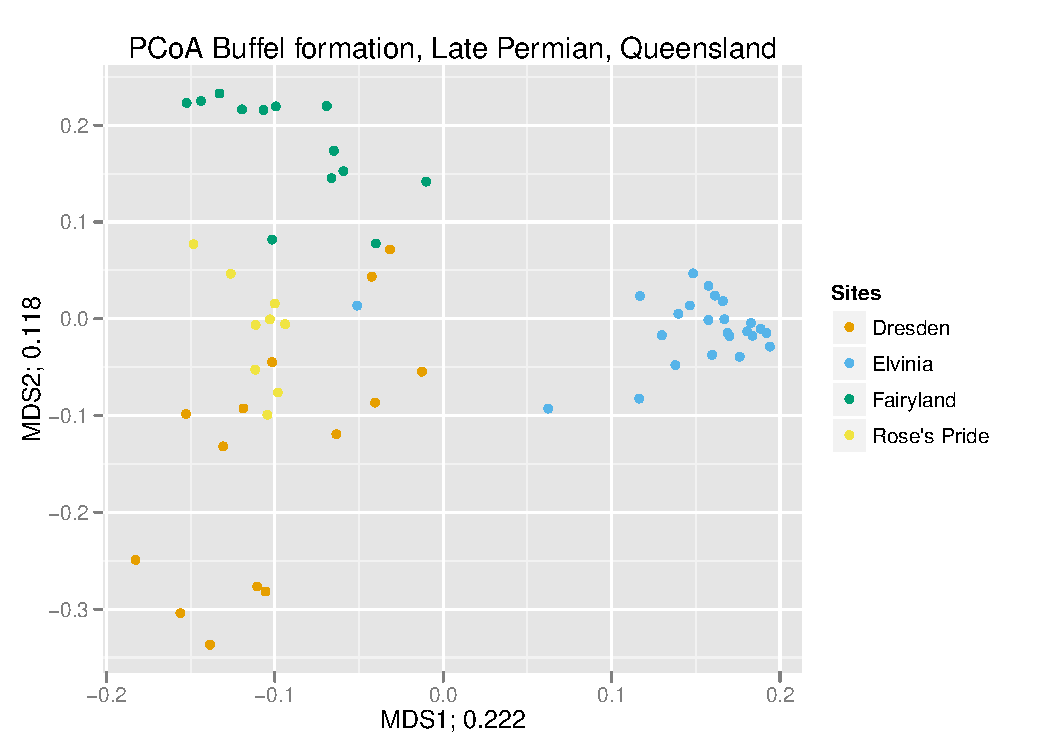
\includegraphics[width=\maxwidth]{figure/buffel-pcoa} 
\end{knitrout}


\end{frame}


\begin{frame}
\frametitle{Ordinations}
\large{Remember, look at the higher axes!}
\\~\\
I have not have done that here, but there is always more information beyond the first and second axes.
Explore them and learn the patterns in your data better
\\~\\
Don't use detrended correspondence analysis as your default. It destroys depictions of complex multidimensional gradients. \textbf{Just don't do it.}

\end{frame}


\begin{frame}
\frametitle{Commandment 8}
\textbf{Thou shalt not cluster shamelessly!} 
The world is full of fuzziness and apostasy, not cool, clean Platonic categories. 
But cluster analysis imposes categories on data regardless of whether they're gradiential. 
If the clusters are really there, thou shalt see them as a ray of divine light in the shadowy purgatory of a multivariate ordination space. 
So why bother?
\end{frame}



\begin{frame}
\frametitle{Clustering}

\begin{knitrout}
\definecolor{shadecolor}{rgb}{0.969, 0.969, 0.969}\color{fgcolor}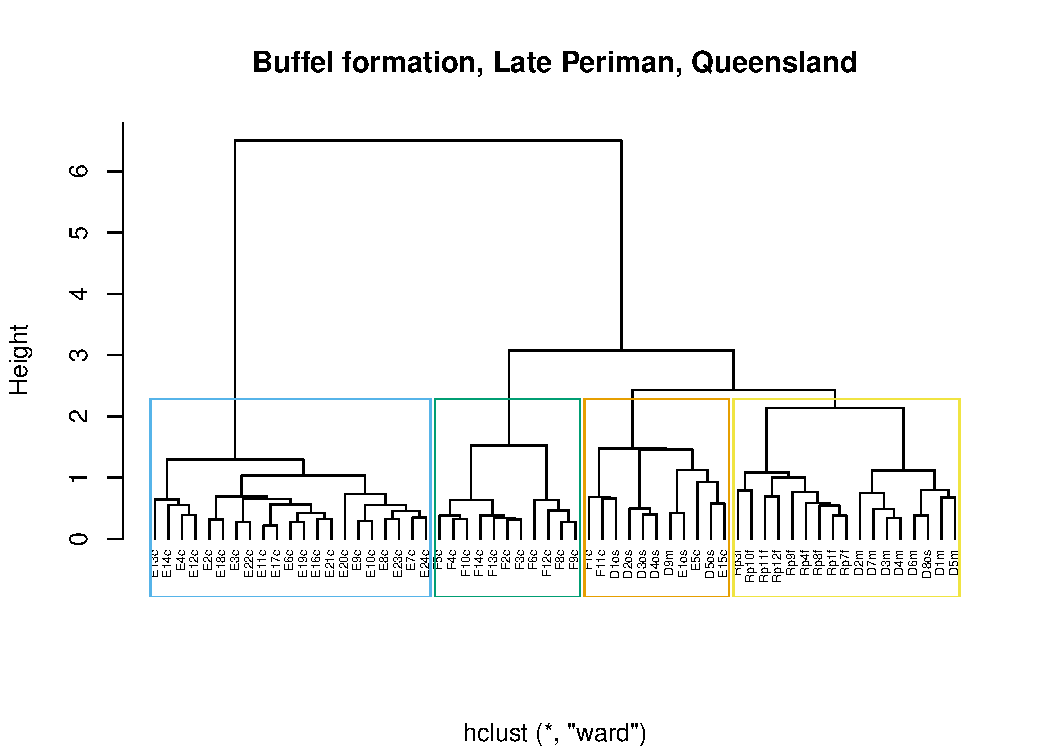
\includegraphics[width=\maxwidth]{figure/cluster} 
\end{knitrout}


\end{frame}


\begin{frame}
\frametitle{Commandment 9}
\textbf{Thou shalt stand awe-struck before the shining brilliance of the G-test!} 
Chi-square this, chi-square that. 
The G is easier to compute, it doesn't blow up as easily because of small values, it depends on the awesome power of the log transform, it stands for ``GOD,'' and most importantly it's a maximum likelihood ratio...
\end{frame}


\begin{frame}
\frametitle{}
G-test now appears in Sokal and Rohlf's ``Biometry''
\\~\\
Also, this makes more sense in the context of...
\end{frame}


\begin{frame}
\frametitle{Commandment 10}
\textbf{Thou shalt sing the praises of likelihood, not ``fit''!} 
Anyone can design another fit statistic. 
Why minimize the sum of squares instead of the sum of cubes or just the sum of differences? 
None of this has a theoretical basis without a notion of probability, and specifically of likelihood. 
After all, that's what the divine theologian Popper said.
\end{frame}


\begin{frame}
\frametitle{Likelihood}
% fit versus likelihood
Fundamental part of all statistical inference. 
\begin{center}
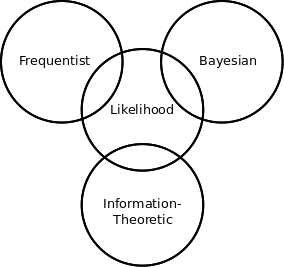
\includegraphics[height = 0.3\textheight]{stat_schools}
% from labstats.net
\end{center}

Measure of how much support our sample gives for some parameter estimate.
Technically always a function, but we are normally most interested in the \emph{maximum} likelihood.
\begin{center}
\begin{math}
L(\hat{\theta} \mid x, model)
\end{math}
\end{center}

\end{frame}


\begin{frame}
\frametitle{AIC}
Approximation of the Kullbach-Leibler divergence for unknown reality.
``What?'' I hear you say...
\\~\\
\small{Incidentally, residual sum squares are a maximum likelihood estimator when the residuals are normally distributed \ldots}
\end{frame}



\begin{frame}
\frametitle{K-L divergence}

K-L divergence is the ``distance'' (not technically a distance) between a reference probability distribution \(f\) (also known as reality) and an approximating probability distribution \(g\).
\\~\\
\begin{math}
I(f,g) = \sum_{i=1}^{k} p_i \cdot \log(\frac{p_i}{\pi_i})
\end{math}
\\~\\
\begin{math}
I(f,g) = \int f(x)\log(\frac{f(x)}{g(x \mid \theta)})
\end{math}
\\~\\
Two of the three fundamental formula in information theory along with Shannon's entropy.

\end{frame}



\begin{frame}
\frametitle{back to AIC}
Akaike showed that the relative expected K-L divergence and the log of the maximum likelihood are related.
\\~\\
\begin{math}
AIC = -2\log(L(\hat{\theta} \mid x)) + 2K
\end{math}
\\~\\
The lowest AIC among the candidate models is the ``closest'' to the unknown reality, with some caveats.
\\~\\
Likelihood is extremely powerful.

\end{frame}


\begin{frame}
\frametitle{}
\huge{Hallelujah!}
\\~\\
\small{but wait, there's more\!}
\end{frame}


\begin{frame}
\frametitle{Peter's first words of advice}
\textbf{Release your source!}
Never underestimate the necessity of reproducible research and analysis.
Using a markup language like {\LaTeX} and  literate programming tools you can embed code in reports, papers, and websites so that anyone, including yourself, can reproduce the exact results with minimal effort.
So find a source repository and release your source to the world.
The less time people expend trying to reproduce your work means more time spent extending and improving your initial offering.
By making your steps more open, you are more accountable for your work and thus a better scientist.
\end{frame}


\begin{frame}
\frametitle{Literate programming?}

\begin{columns}
\begin{column}{0.55\textwidth}
Donald Knuth: 
\begin{quote}
The main idea is to regard a program as a communication to human beings rather than a set of instructions to a computer.
\end{quote}
\end{column}
\begin{column}{0.45\textwidth}
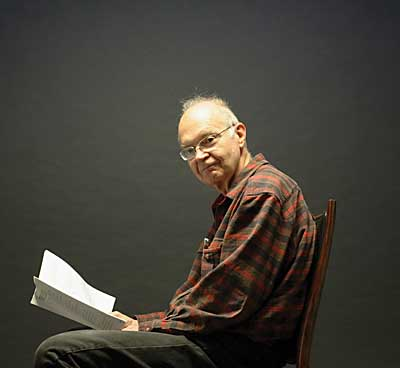
\includegraphics[width = \textwidth]{knuth}
\end{column}
\end{columns}
\end{frame}


\begin{frame}
\frametitle{Tools for R}
\begin{columns}
\begin{column}{0.5\textwidth}
\begin{itemize}
\item Sweave
\begin{itemize}
\item {\LaTeX}
\item old-school
\item mandatory for writing R help files
\end{itemize}
\item knitr
\begin{itemize}
\item {\LaTeX} and markdown
\item shiny new thing designed for dynamic report generation
\item used to write this presentation
\end{itemize}
\end{itemize}
\end{column}
\begin{column}{0.5\textwidth}
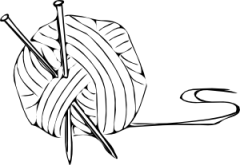
\includegraphics[width = 0.7\textwidth, keepaspectratio = true]{knit-logo}
% image is from the knitr page
% http://yihui.name/knitr/
\end{column}
\end{columns}
\end{frame}


\begin{frame}
\frametitle{Source repository?}
Server to host your source and use version control information at the same time.
\\~\\
I like github.
\\~\\
\begin{center}

\includegraphics[height = 0.4\textheight]{original}
\end{center}

Other options exist like sourceforge, Google Code, R-Forge, etc.
\end{frame}


\mode<all>
{
\usebackgroundtemplate{\centering 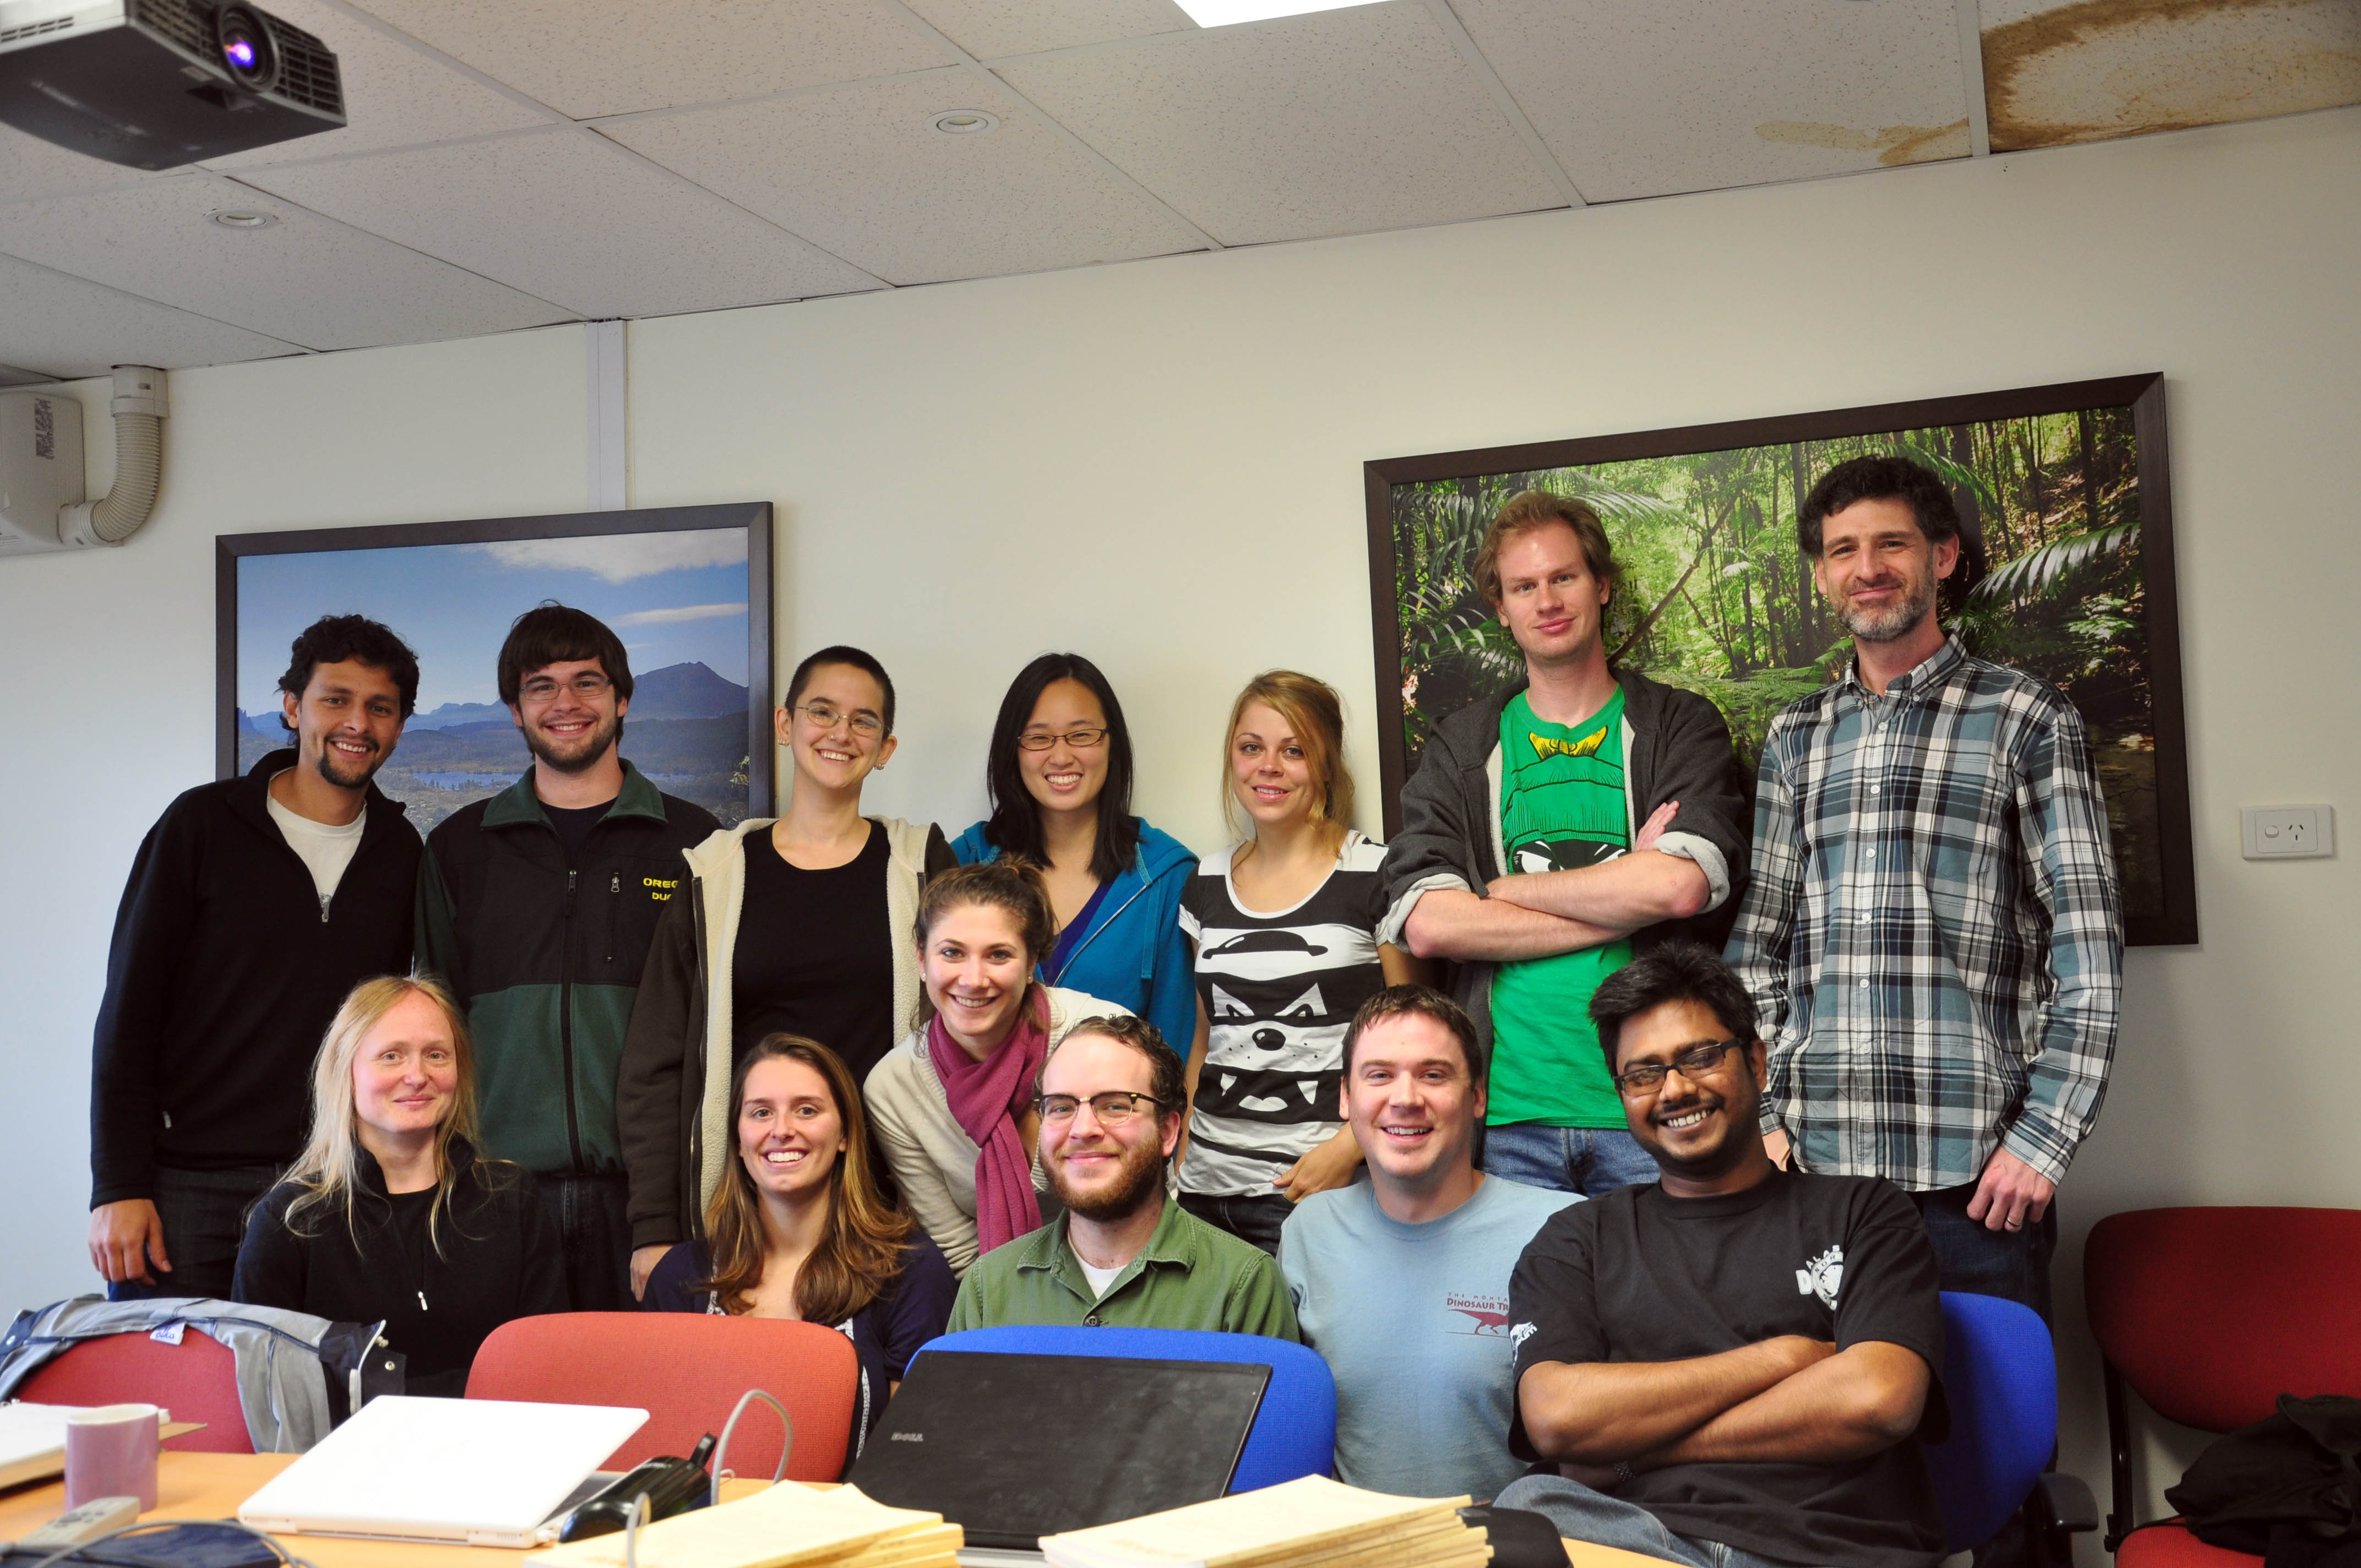
\includegraphics[width=\paperwidth]{alroy_group}}
\begin{frame}[plain]
\end{frame}
}
\mode<all>{\usebackgroundtemplate{}}
\mode*


\begin{frame}
\frametitle{Thanks!}
\begin{columns}
\begin{column}{0.5\textwidth}
\begin{itemize}
\item Alistair Evans
\item Roger Close
\item G10 and all the grad students
\item Ross and Patrick
\item PBDB instructors
\begin{itemize}
\item \textbf{John Alroy}
\item Gene Hunt
\item Tom Olszewski
\item Peter Wagner
\item P. David Polly
\end{itemize}
\end{itemize}
\end{column}
\begin{column}{0.5\textwidth}

\includegraphics[width = \textwidth]{palio_bio}
\end{column}
\end{columns}
\end{frame}


\end{document}
